\section{Motivation}

\logo{}

\begin{frame}{Forecast combination - point and density}

    Combining multiple forecasts can dramatically improve the accuracy of the forecast (\cite{BG69}).
    
    \vspace{5mm}

    
    Point Forecast Combination 
    \[\hat y_t = \omega \ \hat y_{1t} + (1-\omega) \ \hat y_{2t}\]

    Density Forecast Combination
    \[ \hat f(y_t) = \omega \ \hat f_1(y_t) + (1-\omega) \hat f_2(y_t)\]

\end{frame}


\begin{frame}{Forecast combination puzzle}

\begin{columns}[t]
    \begin{column}{0.5\textwidth}
        \centering
        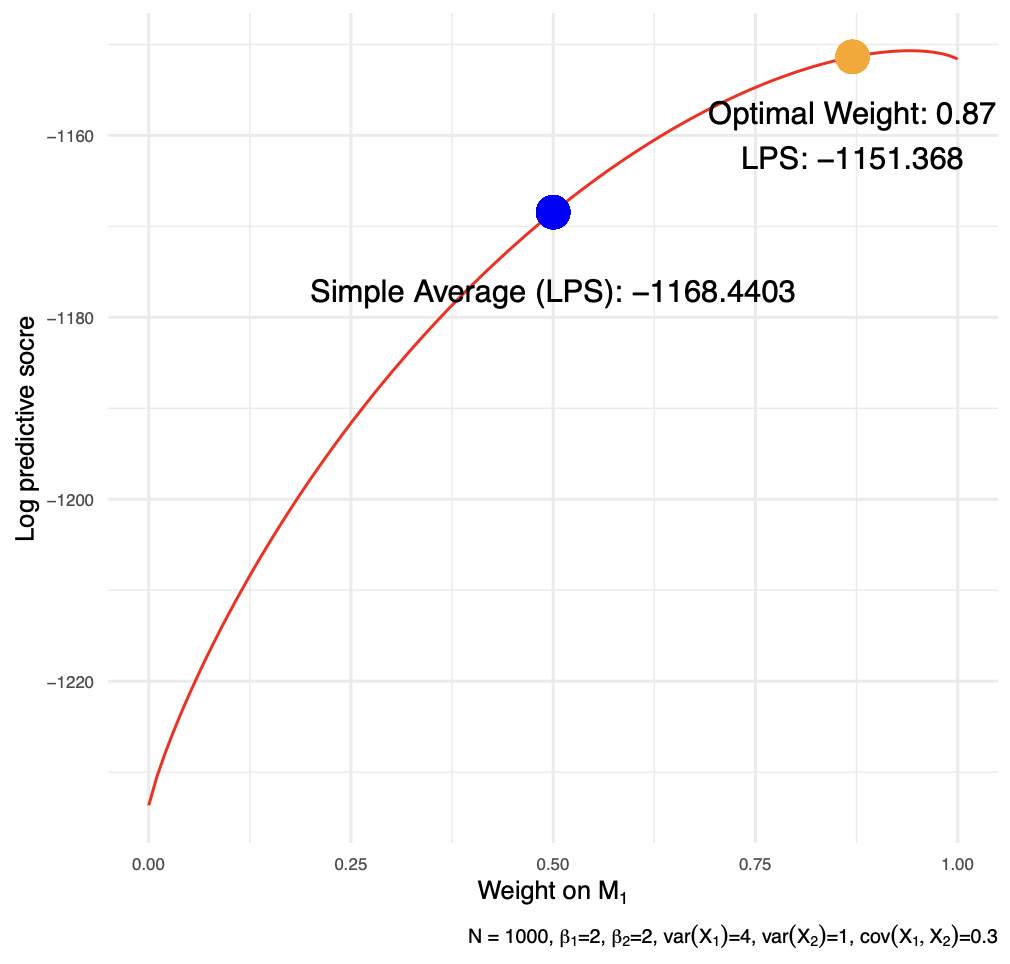
\includegraphics[width=6cm]{Graph/Ex1.png}
    \end{column}
    
    \begin{column}{0.5\textwidth}
        \centering
        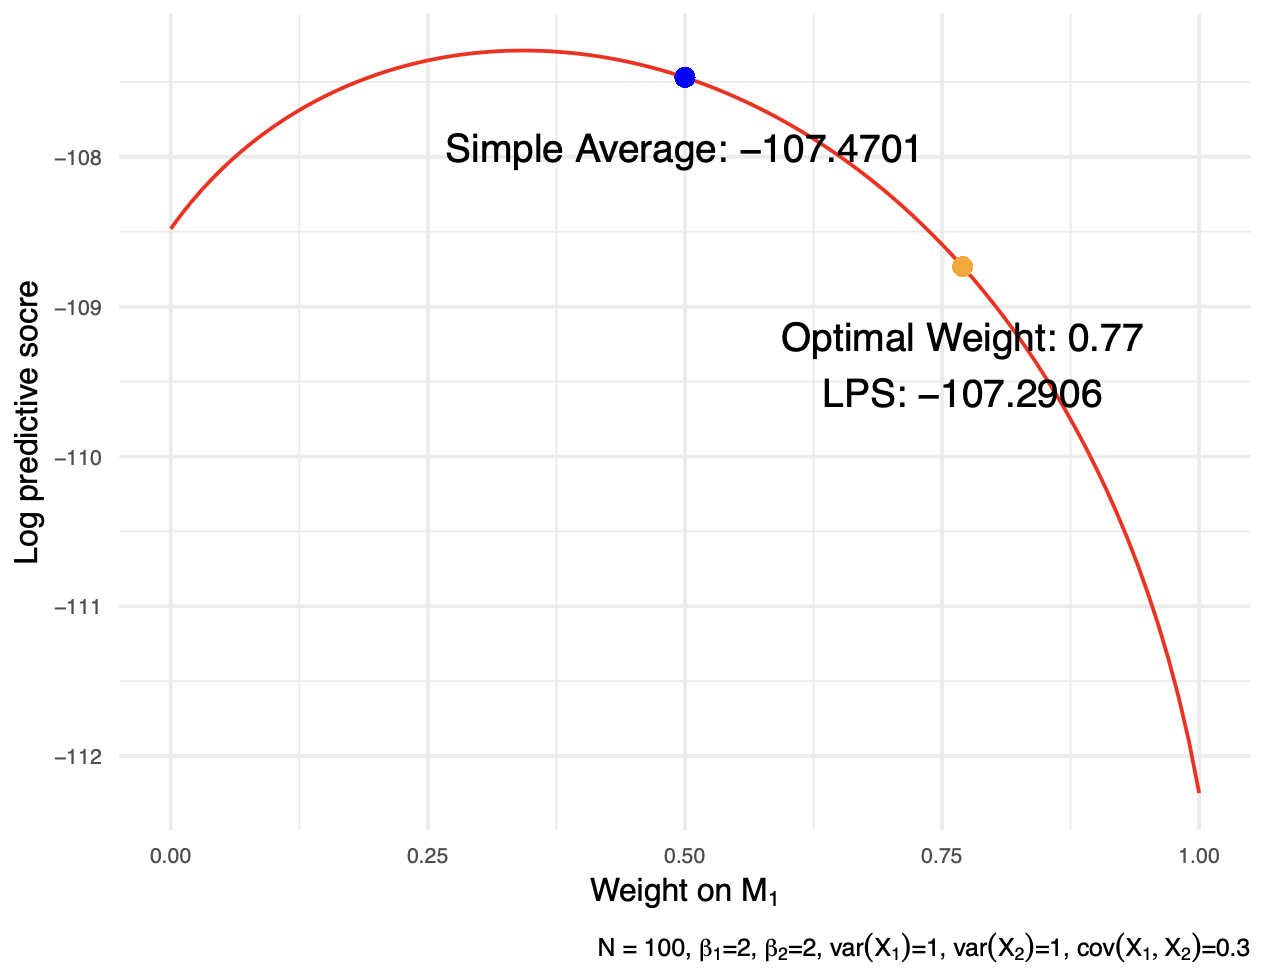
\includegraphics[width=6cm]{Graph/Ex2.png}
    \end{column}
    \end{columns}

    \vspace{-6mm}
    
    \begin{columns}[t]
    \begin{column}{0.5\textwidth}
        \begin{alertblock}{}
        \centering
        \tikz{\fill[orange] circle (3pt);} \ Complicated Weighting Schemes
        \end{alertblock}
    \end{column}
    
    \begin{column}{0.5\textwidth}
        \begin{exampleblock}{}
        \centering
        \tikz{\fill[blue] circle (3pt);} \ Simple Averaging
        / Equal Weights
        \end{exampleblock}
    \end{column}
    \end{columns}

\end{frame}



\begin{frame}{When should we expect the puzzle}

    In the linear regression context, the optimal weight $\hat\omega_{opt}$ has a closed-form expression when using the Mean Squared Error (MSE) weighting scheme.
    
    
    \[\hat\omega_{opt} \overset{p}{\to} \omega_\star = \frac{\alpha_1'\Sigma_{11}\alpha_1 - \alpha_1'\Sigma_{12}\alpha_2}{\alpha_1'\Sigma_{11}\alpha_1 - 2\alpha_1'\Sigma_{12}\alpha_2 + \alpha_2'\Sigma_{22}\alpha_2}\]


    The presence of the puzzle is tightly related to the coefficients and the variances of regressors in both proposed models.
    
    
    \[\omega_\star=\frac{1}{2} \Rightarrow \alpha_1'\Sigma_{11}\alpha_1 = \alpha_2'\Sigma_{22}\alpha_2\]

    In-sample performance

    
\end{frame}



\begin{frame}{Preliminary Conjecture}

    Consider a two-model combination.

    \begin{table}[ht]
    \centering
    \begin{tabular}{cccc}
                           &      & \multicolumn{2}{c}{$M_2$} \\
                           &      & Good       & Bad       \\
    \multirow{2}{*}{$M_1$} & Good & \alt<2>{\color{MonashBlue} $\surd$}{$\surd$}    & \alt<2>{\color{Orange} $?$}{$?$} \\
                           & Bad  & \alt<2>{\color{Orange} $?$}{$?$}        & \alt<2>{\color{MonashBlue} $\surd$}{$\surd$}
    \end{tabular}
    \label{tab:1}
    \caption{\footnotesize Initial conjecture on the presence of forecast combination puzzle}
    \end{table}
    
    The in-sample fit between two models in a relative sense may indicate the presence of the puzzle.


\end{frame}



\begin{frame}{Preliminary Conjecture}
\centering
\begin{tikzpicture}
    \draw[step=1cm,gray,very thin];
    \draw[thick,->] (0,0) -- (7,0);
    \draw[thick,->] (0,0) -- (0,5);
    \draw[thick,->] (0,0) -- (7,0) node[anchor=north west] {$M_1$ LogL};
    \draw[thick,->] (0,0) -- (0,5) node[anchor=south east] {$M_2$ LogL};
    
    \foreach \Point in {(1,1), (2,2), (3,3), (4,4)}{
    \node [MonashBlue] at \Point {$\surd$};}
    
    \foreach \Point in {(6,2), (5,1), (1,4), (2,5)}{
    \node [Orange] at \Point {$?$};}

    \foreach \Point/\PointLabel in {(6,2)/GB, (5,1)/GB, (1,4)/BG, (2,5)/BG}
        \draw[fill=Orange] \Point circle (0.0005) node[above right] {\color{Orange} \PointLabel};
\end{tikzpicture}

\end{frame}





